\section{Auswertung}
\label{sec:Auswertung}

\subsection{Fehlerrechnung}
  Zur Fehlerrechnung werden die Fehlerpfortpflanzung nach Gauß

  \begin{equation}
    \sigma_f = \sqrt{ \left( \frac{\partial f}{\partial x} \right)^2 \sigma_x^2 + \left( \frac{\partial f}{\partial y} \right)^2 \sigma_y^2 }
  \end{equation}

  und die Standardabweichung vom Mittelwert

  \begin{equation}
    \sigma_{\bar{x}} = \sqrt{ \frac{1}{N \left(N-1 \right)} \sum_{k=1}^{N} \left(x_k - \bar{x} \right)^2 }
    \label{Fehler:1}
  \end{equation}

  mit

  \begin{equation}
    \bar{x} = \frac{1}{N} \sum_{k=1}^{N} x_k
    \label{Fehler:2}
  \end{equation}

  verwendet.

\subsection{Überprüfung der Stabilitätsbedingung}
  Als erstes wird die Stabilitätsbedingung untersucht. Der Laser ist stabil wenn

  \begin{equation}
    0 \le g_1 \cdot g_2 < 1
    \label{Eqn:1}
  \end{equation}

  gilt. Die Resonatorparameter werden nach

  \begin{equation}
    g_i = 1 - \frac{L}{r_i}
    \label{Eqn:2}
  \end{equation}

  berechnet. In Abbildung \ref{Abb:1} werden die theoretischen Kurven der drei
  Anordnungen dargestellt.

  \begin{figure}
    \centering
    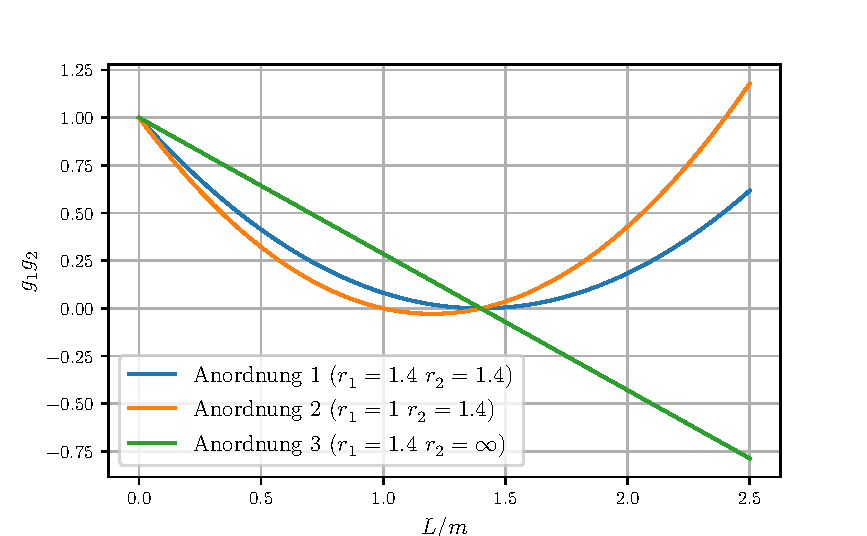
\includegraphics[width=\textwidth]{Anordnungen_Theorie.pdf}
    \caption{Theoretische Stabilitätsbedingung für die drei Anordnungen.}
    \label{Abb:1}
  \end{figure}

  Experimentell wurden die Werte der Anordnung 1 und 3 gemessen. Dabei ergaben
  sich für $L_1$ und $L_3$ folgende Werte:

  \begin{align}
    L_1 &= 138.9\,\text{cm} \\
    L_3 &= 102.8\,\text{cm}
  \end{align}

\subsection{TEM-Moden}
  \subsubsection{TEM$_{00}$-Mode}
    Die Intensitätsverteilung der TEM$_{00}$-Mode kann als Gaußverteilung der
    Form

    \begin{equation}
      I_{00}(r) = I_0 \cdot \text{exp} \left(\frac{2 r^2}{\omega^2} \right)
      \label{Eqn:3}
    \end{equation}

    dargestellt werden. Die Messwerte der Intensitätsverteilung sind in Tabelle \ref{tab:1}
    dargestellt.

    \begin{table}[h]
\centering
\caption{Intensitätsverteilung der TEM$_{00}$-Mode in Abhängigkeit zum Abstand.}
\sisetup{%uncertainty-seperator = {\,},
table-number-alignment = center,
table-unit-alignment = center,
%table-figures-integer = 1,
%table-figures-decimal = 1,
table-auto-round = true
}
\begin{tabular}{S[table-format= 1.3]
  S[table-format= 1.3]
  S[table-format= 1.3]
  S[table-format= 1.3]
  S[table-format= 1.3]
  S[table-format= 1.3]
  S[table-format= 1.3]
  S[table-format= 1.3]
  S[table-format= 1.3]
  S[table-format= 1.3]
  }
\toprule
{$r \text{ in mm}$}
&{$I(r) \text{ in $\mu$A}$}\\
 \midrule
 0.0&0.013\\
 0.5&0.260\\
 1.0&0.950\\
 1.5&0.950\\
 2.0&1.880\\
 2.5&2.500\\
 3.0&2.400\\
 3.5&1.300\\
 4.0&0.400\\
 4.5&0.090\\
\bottomrule
\end{tabular}
\label{tab:1}
\end{table}

